\documentclass[12pt, letterpaper]{article}
\usepackage{amsmath}      % For advanced math, gather, align, and cases
\usepackage{amssymb}      % For mathematical symbols
\usepackage{graphicx}     % For including images
\usepackage{subcaption}   % For subfigures (Layout 6.1)
\usepackage{multirow}     % For multirow table cells
\usepackage{makecell}     % For multi-line text inside a single table cell
\usepackage{physics} % \dv, \pdv, \ket (optional)

\graphicspath{{images/}}
\title{My first LaTeX document}
\author{Hubert Farnsworth\thanks{Funded by the Overleaf team.}}
\date{August 2022}
\begin{document}
\maketitle
Hello \\ World
\begin{figure}[h]
    \centering
    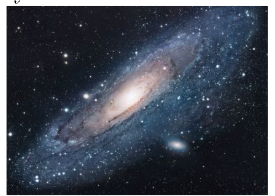
\includegraphics{universe.png}
    \caption{\textbf{\textit{What are we doing}}}
    \label{universe}
\end{figure}

As you can see in figure \ref{universe} is there. The example is on page \pageref{universe}.

Hello
\[\frac{a}{b}\]
\end{document}

